\documentclass{article}
\usepackage{preamble}
\usepackage{dirtree}

\title{Classroom Response Systems in IT classrooms}
\author{Jonas Tonny Nielsen \and Jonas Lomholdt}
\date{\today}

\begin{document}

\maketitle

\begin{abstract}
    Lorem ipsum dolor sit amet, consectetur adipiscing elit. Donec a diam lectus. Sed sit amet ipsum mauris. Maecenas congue ligula ac quam viverra nec consectetur ante hendrerit. Donec et mollis dolor. Praesent et diam eget libero egestas mattis sit amet vitae augue. Nam tincidunt congue enim, ut porta lorem lacinia consectetur. Donec ut libero sed arcu vehicula ultricies a non tortor. Lorem ipsum dolor sit amet, consectetur adipiscing elit. Aenean ut gravida lorem. Ut turpis felis, pulvinar a semper sed, adipiscing id dolor. Pellentesque auctor nisi id magna consequat sagittis. Curabitur dapibus enim sit amet elit pharetra tincidunt feugiat nisl imperdiet. Ut convallis libero in urna ultrices accumsan. Donec sed odio eros. Donec viverra mi quis quam pulvinar at malesuada arcu rhoncus. Cum sociis natoque penatibus et magnis dis parturient montes, nascetur ridiculus mus. In rutrum accumsan ultricies. Mauris vitae nisi at sem facilisis semper ac in est.
\end{abstract}

\tableofcontents

\listoffigures

\listoftables

% ===== TODOS ======
\clearpage
\listoftodos
\clearpage
% ===== END TODOS ======


% ===== SECTIONS ======
\todo{Introduction}
Skal omskrives, rettes og tilpasses



\todo{Lav abbreviation list} \clearpage
\section{Introduction}
During recent years, a number of studies have shown how introducing clicker systems, also known as Classroom Response System (CRS), can have a positive effect on learning outcomes and classroom interactivity \cite{yourstone2008classroom, siau2006use, lantz2014effectiveness}.

The idea of CRSs is not a new one, and low tech paper based versions have been used in classrooms before. The system is simple, where students hold up a piece of paper, called a response card, with their answer \cite{ralph1994effects}. During the last decade more modern versions of this system has been introduced, the so called \emph{clickers}. A clicker in it's most basic form, is a device that allows the users to respond to questions, most commonly in a classroom environment. Such a system has been defined by \citeA{lantz2014effectiveness} as 

\begin{quote}
    \emph{"[...] individual response devices held by individual students allowing them to quickly and anonymously respond to multiple choice questions presented in class. A receiver attached to a classroom computer collects and summarizes the responses instantly and projects them graphically onto the screen for students and the educator to see"} \cite[p.~280]{lantz2014effectiveness}
\end{quote}

As described above, the clicker itself is used for gathering collective answers from the students via a physical clicker device. Many different versions of such systems exists\footnote{\url{https://www1.iclicker.com/}, \url{http://www.renaissance.com/products/2know}}. One example of such a system can be seen in figure \ref{fig:iclicker}.

\begin{figure}[H]
\capstart
	\centering
		\frame{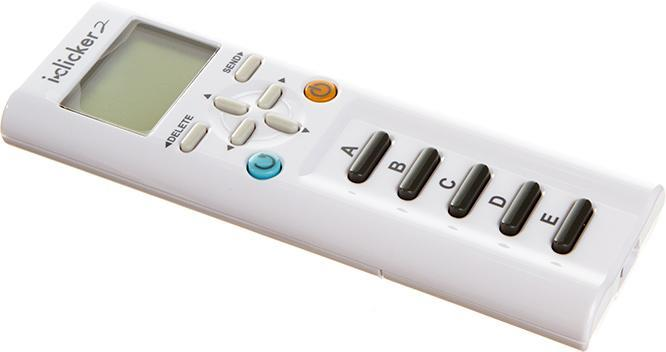
\includegraphics[width=\textwidth]{iclicker.jpg}}
        %\missingfigure{iClicker - An example of an iClicker}
	\caption[iClicker2]{One example of a clicker device called the iClicker2.}\label{fig:iclicker}
\end{figure}

The device depicted in figure \ref{fig:iclicker} is a hardware based CRS, that connects to a receiver in the classroom, that is connected to the teachers computer. The computer can then display the data with a piece of software designed for the system.

A typical hardware based CRS system like the one mentioned above introduces a variety of pros and cons. This includes the investment of buying the system, the receiver and possible licenses for using it could become a large expense. Also there are potential risks, that setting up the system could become a hassle, if the software for example is not maintained for more than one platform or the hardware is difficult to setup. With the emerging of smartphones and fast, reliable internet connections, it could seem like a natural progression to utilize the devices that the users already own, cutting away the expense of buying clicker devices. The users would then use their smartphones or laptops to respond, instead of using a clicker. The concept has been dubbed \emph{Bring Your Own Device} or \emph{BYOD} \cite<Johnson et al., 2013 in>[p.~329]{stowell2015use}. Such systems exists in a variety of different forms, implemented with mixed results. Making the move from the physical to a digital based platform, introduces a whole new range of possibilities and challenges.

There are a variety of examples of online CRS systems. Some are made mainly for children or ground-schoolers\footnote{\url{https://kahoot.it}}, and others are feature rich, made for conferences and classrooms\footnote{\url{http://socrative.com}} \footnote{\url{https://www.polleverywhere.com}} \footnote{\url{https://www.iclicker.com/}}. The most appealing, and seemingly well implemented system is Mentimeter\footnote{\url{https://www.mentimeter.com}}.

Much of the available existing literature about CRS is focused on physical clicker devices and the learning outcomes/improvements of using them. It's less common to find research where the main focus is web based systems, even though smartphones has become widespread and more popular among students \cite[p.~329]{stowell2015use}.

Our own experience shows that it can be problematic when the teacher wants to ask questions which include code. This is hard to do on hardware based devices, and different workarounds where questions are asked on slideshows and answered on clickers are common. We will therefore develop a system that supports showing code and math and test whether or not it's capable of increasing interaction and improving the learning outcome. The research question of this project is:

\begin{quote}
We wish to investigate whether a Classroom Response System that is enhanced for IT educational purposes, is able to enhance classroom interactivity and thereby increase the learning outcome. 
We wish to evaluate the system by gathering empirical data by conducting a pre and post survey on students using our system.
\end{quote}

We wish to gain knowledge on how the market is structured today. By using Porters Five Forces \cite{porter2008five}, we will identify possible culprits that we should be aware about when creating such a system, for it to be competitive.

We will then describe the system that we have developed in two parts. First a general introduction to the system. Secondly a technical description of the specific implementation.
We will then perform a test in two different courses: \emph{Frameworks and Architectures for the Web} and \emph{Advanced Programming}, and discuss our results from the test and show how each CRS performs compared to each other in the two different courses.



% It would seem that the obvious approach would be to leverage the technology that students already own and use. At the IT University of Copenhagen (ITU), laptops are mandatory and free internet access is provided by the university. 

% Each system has a different focus, and how deeply integrated they are varies. Some systems simply wants to ask questions, others wants to grade assignments or provide feedback as well. Though few of them seem to have focus on IT learning specifically, and the ones implementing features that do, lack in other ways.



 \clearpage
\todo{Det her er det samme som "Background" - måske}\section{Existing literature and solutions} % What is already known and done + existing solutions?

%%% Some intro to this maybe...
In this section we will describe different studies and findings from existing literature in order to provide insights of the field of classroom response systems. These insights will help us understand how previous work has been done and how we can evaluate our solution. Furthermore, we will include a description of significant existing solutions in order to compare their features. This comparison will tell us what's missing from existing solutions and which problems we will address.


\subsection{Literature and research} %about CRS}

The following section will include findings, results and mentions of some of the most significant research in the field of response systems in classrooms. Furthermore, this section will mention research based response systems developed at MIT and University of Lugana.

Some of the least resent literature dating back to around 2007, is mainly focused on physical clicker devices, where the students buy actual "remote controls" for polling, in a time where more modern solutions (including the smartphone) has not yet matured. And even today, the physical clicker devices still seem to play a significant role in the \emph{"clicker community"}. \citeA{stowell2015use} explains how the use of clicker systems on physical devices has a greater response rate compared to mobile, but with no significant differences in the final grades of the students. Also, the introduction of students bringing their own devices (the so called \emph{Bring Your Own Device}) introduces new issues such as loss of internet connectivity and the risk of being distracted by the device itself (pp. 331-332).


One of the main reasons to use a CRS is the importance of interactivity in learning \cite{draper2004increasing}. Studies find that CRS engages interactivity, helps students stay active during lectures \cite[p.~116]{moredich2007engaging}, improves learning \cite<e.g.,>{siau2006use, yourstone2008classroom} and increases attention \cite[pp.~86-88]{sun2014influence}. While \citeA{yourstone2008classroom} focuses on actual results in learning outcomes and \citeA{sun2014influence} uses brainwave analysis to determine level of attention while using CRS, most other studies take on a qualitative approach and evaluate teachers and students by asking to their engagement, participation and learning outcomes \cite<e.g.,>{moredich2007engaging}. The latter approach seems to be the most widespread in the literature and focuses more on whether or not students feel an increased engagement and participation rather than their actual performance and examination results. 


\citeA{stowell2007benefits} takes on the qualitative approach where they ask into students emotions towards an introductory psychology class before, during and after lecture. The study compares standard lectures to hand raising, response card and "clicker" lectures\footnote{Standard lectures are thought of as normal lectures where the teacher asks open ended questions to the students. Hand raising is the approach where students are asked to raise their hand if they agree to a statement. Response cards are cards labeled A, B, C, D and are sort of the same as hand raising \cite[p.~254]{stowell2007benefits}.}.
They find that more correct answers to questions are present in response card lectures but explains the much higher correctness with the ability to see what peers are answering \cite[p.~257]{stowell2007benefits}. The same applies for hand raising. Furthermore the study finds that there's a small positive impact on emotions towards the class depending on which kind of lecture is taught (i.e. standard, hand raising, response card and "clicker") \cite{stowell2007benefits}.

One study found that there wasn't a framework for measuring interactivity in classrooms \cite[p.~400]{siau2006use}. They then designed a test framework which consists of a \emph{pretest}, \emph{implementation}, \emph{posttest} and \emph{qualitative data collection}. The pretest is done before starting using a classroom response system. The posttest asks the same questions as the pretest which are then compared to measure difference in interactivity. The posttest, which is done at the end of the course, asks further into the technology and the response system used in the classroom and how the it's perceived \cite{siau2006use}. The implementation is simply the implementation of the response system in the class which are done after the pretest. Finally, the qualitative data collection asks into advantages and disadvantages of using a response system. Their study found a significantly increased interaction reported by the students who participated \cite[p.~400]{siau2006use}. The increase measured on an individual and general level. 


Among the biggest studies of CRS is \emph{Increasing interactivity in lectures using an electronic voting system} by \citeA{draper2004increasing}. This particular study took place over a two year period and found (among other things) that the benefits increases as teachers became aware how to exploit the pedagogy behind the system \cite[p.~93]{draper2004increasing}. The study took place in a time where there was a need for physical hardware (e.g., remote controllers and receivers) in order to facilitate a CRS. This study addresses the need to learn how to proper use a CRS in order to get the benefits from it.

The next parts will focus on some articles which describes and study some different kind of response systems. The studies take on different approaches at teaching computer science and the response systems include atypical features.

All of the before mentioned studies have either not specified which system was used or they used one of the traditional systems available such as the iClicker. Another type of CRS we've found called \emph{Informa} focuses mainly on teaching Java \cite{Hauswirth09}. The system is a software based solution made in Java. The system consists of two different clients; an instructor client and several student clients \cite[p.~1]{Hauswirth09}. Informa is different because it's not a traditional response system, but a task based peer-grading system where the instructor creates a task which the students then are supposed to solve. Students who finish early can grade other students solutions while waiting for everyone to finish \cite{Hauswirth09}. One of \citeA[p.~9]{Hauswirth09}'s findings are that students find the system useful but it's unsure if the system is more useful for the weaker or stronger students. \emph{Informa} is worth mentioning because it is not a typical response system and because it bridges the gap between classroom response systems and teaching a programming language. However, it seems to be limited to teaching Java and can thus not be used to teach other type of courses.

A similar approach can be found in the pen-and-tablet based system that has been used to teach introductory computer science at MIT \cite{koile2007supporting}. The system is called \emph{Classroom Learning Partner} and is a response system where the students answer to question by writing with a pen on a tablet. The hand-written answer is recognized and interpreted by the system, but not without difficulties \cite[pp.~2-3]{koile2007supporting}. A previous study found that their system could improve learning in a CS1 (Computer Science 1) class \cite{koile2006improving}. The study introduced one of two classes to the tablet based system after the first exam (in week 5 of 15) \cite[pp.~6-7]{koile2006improving}. The class not using the system functioned as control group \cite[pp.~6-7]{koile2006improving}. By comparing the score of the students in the different classes their preliminary results showed a difference between the two, where the tablet-PC class performed slightly better \cite{koile2006improving}. They also report that fewer than expected students performed poorly in the tablet-PC class, where \emph{"23.5\% of non-Tablet-PC students were in the bottom 25\% of the class, vs. 6.0\%."} \cite[p.~7]{koile2006improving}. % The significance was p < .05. \clearpage
\section{Method}



The idea of Classroom Responses Systems is not a new one. As mentioned, early analog versions of these systems where used where students simply raised a card with their answer \cite[p.~257]{stowell2007benefits}. Several examples of such systems in more moderns versions have been shown, and such we must determine where our system lies from a strategic standpoint. To find this out we have used our own interpretation of \emph{Porters Five Forces} \cite{porter1979competitive}.


\subsection{Porters Five Forces}
The model shows how competition can be seen as five forces. 

\emph{The threat of new entrants}, how new entrants to an industry have a desire to gain market share. \emph{The bargaining power of suppliers}, the dynamics of suppliers changing prices and capturing more value for themselves. \emph{The bargaining power of buyers}, the fact that buyers can demand more value by forcing down prices or wanting better quality. \emph{The threat of substitues}, other products on the market offering the same or better products by different means. For example using LearnIT's native question feature instead of using a dedicated CRS. And finally, the fact that other systems compete for market share already, introducing new features or discounted pricings. Figure \ref{fig:porter5forces} shows a depiction of the model as it is explained in \citeA[p.~141]{porter1979competitive}. 

% Threat of New Entry
% Supplier Power
% Threat of Substitution
% Buyer Power
% CENTER: Competitive Rivalry
% https://www.mindtools.com/pages/article/newTMC_08.htm

\begin{figure}[H]

\centering
\begin{tikzpicture}
[node distance = 1cm, auto,font=\footnotesize,
% STYLES
every node/.style={node distance=3cm},
% The comment style is used to describe the characteristics of each force
comment/.style={rectangle, inner sep= 5pt, text width=4cm, node distance=0.25cm, font=\scriptsize\sffamily},
% The force style is used to draw the forces' name
force/.style={rectangle, draw, fill=black!10, inner sep=5pt, text width=4cm, text badly centered, minimum height=1.2cm, font=\bfseries\footnotesize\sffamily}] 

% Draw forces
\node [force] (rivalry) {Rivalry among existing competitors};
\node [force, above of=rivalry] (substitutes) {Threat of substitutes};
%\node [force, text width=3cm, dashed, left=1cm of substitutes] (state) {Public policies};
\node [force, left=1cm of rivalry] (suppliers) {Bargaining power of suppliers};
\node [force, right=1cm of rivalry] (users) {Bargaining power of users};
\node [force, below of=rivalry] (entrants) {Threat of new entrants};

%%%%%%%%%%%%%%%
% Change data from here

% RIVALRY
\node [comment, below=0.25 of rivalry] (comment-rivalry) {
%(+) A war against Microsoft\\
%(+) Limiting sunk costs\\
%(+) Coopetition
};

% SUPPLIERS
\node [comment, below=0.25cm of suppliers] {
%(+) Efficiency\\
%(+) Attracting other developers\\
%(+) Creating a Chrome community
};

% SUBSTITUTES
\node [comment, right=0.25 of substitutes] {
%(+) Portability
};

% USERS
\node [comment, below=0.25 of users] {
%(+) Increasing the user information\\
%(+) Reducing the switching costs
};

% NEW ENTRANTS
\node [comment, right=0.25 of entrants] {
%(+) EC vs. Microsoft
};

% PUBLIC POLICIES
%\node [comment, text width=3cm, below=0.25 of state] {
%(+) Positively framed\\
%(+) Transparency\\
%(--) A new monopoly?
%};

%%%%%%%%%%%%%%%%

% Draw the links between forces
\path[->,thick] 
(substitutes) edge (rivalry)
(suppliers) edge (rivalry)
(users) edge (rivalry)
(entrants) edge (comment-rivalry);

\end{tikzpicture} 
\caption{Porters Five Forces }\label{fig:porter5forces}
\end{figure}


All forces must be taken into consideration when evaluating the strategic position to ensure our systems sustainability\todo{Find other word for this?} in a challenging market. 
In the following section we will determine how these forces can be interpreted against our system, and essentially our strategy.

The amount of fully digital CRS systems are manifold. The ones that we mention here is merely the ones that we were able to find by during our research. Arguably there might me more, but we will only be concerned about the ones mentioned here. 


\subsubsection{Threat of new entrants}
We will primarily be focusing on the the seven entry barriers, that incumbents have relative to new entrants, as explained by \citeA{porter2008five}, in relation to our own system.


The first barrier is \emph{supply-side economies of scale}. Essentially it covers the fact that the larger volumes, creates lower cost per unit. This is essentially true, due to the fact that a unit in our sense is users, and our cost per unit is server maintenance cost, the more users, the more servers but also spread fixed costs. For entrants though, the cost can be low and may simply scale as the business expands.

The \emph{demand-side benefits of scale}, is the fact that users might have increased willingness to buy a product if other buyers patronize the company. Users may also value being part of a bigger \emph{network}, thus this barrier is also known as the \emph{network effect} \cite[p.~81]{porter2008five}. It's hard to counter the fact that a huge volume will have a positive effect on almost any platform, but in general with CRS systems, it would seem plausible that systems are chosen based on user needs. This leads us naturally towards the third barrier \emph{customer switching costs}. The name is mostly selfexplanatory, but this barrier regards the switching cost to a new system. If we only consider web based systems, which most of the modern ones are, most users does not have any deep data affiliation with the systems, so switching comes at almost no cost. For entrants this is very positive. Given that gaining traction on such a market is very much possible if the system is feature competitive.

\emph{Capital requirements} consider the fact that th \emph{"need to invest large financial resources in order to compete can deter new entrants"} \cite[p.~81]{porter2008five}. In the case of CRS, it should be possible to build such a system without great capital requirements. In fact a working prototype can be made ready very quickly, as our example shows, thou this is also a threat once you are in the market, potential entrants can be plentiful.

\emph{Incumbency advantages independent of size} take into consideration the fact, that almost any incumbents has the advantage of already being available on the market \cite[p.~81]{porter2008five}. Simply put, being first can have potential advantages. Even though this might seem obvious, it is important to remember while analysing the CRS market. It would seem that many have tried (referring to the many systems mentioned here), and many also appears well established, but none seem to be dominant and.

Entrants and incumbents might have \emph{unequal access to distribution channels}. For entrants, distribution channels must be secured in order to be able to displace others from the market. While dealing with non-physical products, and in this case dealing with software where the "shelf space" is unlimited, the distribution channels  comes down to marketing of the product. Everybody has equal ability to market their product (online for example), but here the capital requirements might come in to play, since marketing can be a costly affair, and the distribution channels depend on it.

The final barrier is \emph{restrictive government policy}. It concerns the fact that the government might have direct influence on whether you will be able to even become an entrant on the market \cite[p.~82]{porter2008five}. Gathering potential licenses or other restrictions that might apply from a government level should be considered. While handling digital systems, laws governing privacy and data security should also be dealt with, though most CRS does not handle much user data beside an email or username and a password which is also the case in our system.


\subsubsection{Bargaining power of suppliers}
The next force is the \emph{bargaining power of suppliers}. This is concerned with the fact that 

\subsubsection{Threat of substitute products or services}


\subsubsection{Bargaining power of buyers}


















\subsection{Test of CRSFIT and design of the test}
We have designed a test in order to tell whether or not our solution can have an impact on teaching classes that covers teaching programming and mathematics. The test is highly inspired by \cite{siau2006use} and their work.

The test is designed to tell whether or not we are able to move peoples behaviour, beliefs and attitude towards engagement, interactivity and participation during class. \citeA{siau2006use} defined a test design consisting of a \emph{pretest}, \emph{implementation} of the system in a class and a \emph{posttest} followed up by a \emph{qualitative data collection} doing exactly this. Our test is structured in the same way and we are asking similar questions in the different parts of the test as well. The whole test should preferably be carried out over a whole semester, but due to the limited time of this project the test will be carried out in a single lecture. The pretest and posttest are made as questionnaires. 

By having a pretest and a posttest asking the same questions we'll be able to compare the results and measure whether or not we are able to move peoples attitude. The pretest consists of two parts which are asking about individual interactivity and general interactivity in the class. We are asking people to answer on a Likert scale from \todo{INSERT REF TO LIKERT SCALE SOMETHING!} 1-9 where 1 is \emph{Strongly disagree} and 9 is \emph{Strongly agree}. The questions in the first part of the pretest (individual) are formulated as statements such as \emph{"I am engaged in class."} and \emph{"I provide my opinion to questions from the teacher during the class."}. In the second part of the pretest (general) we will ask students to answer similar statements such as \emph{"Students participate in class discussion."} and \emph{"Students receive feedback in class on their understanding of the course materials."}. The pretest should be answered by students before or in the beginning of the given lecture in which the test is carried out. \todo{Smid det i appendix?}See \url{https://docs.google.com/forms/d/1Yv3HKuvZYB-y560yfxCAaFkT3WifR7-tyLxM5T5-Zds/edit?usp=forms_home} for a complete version of the pretest questionnaire.

During the lecture, we will ask students questions relevant to their class with our solution, CRSFIT. This part of the test is the \emph{implementation}. Students will answer these questions anonymously and they will not be held accountable for their answers. The purpose of this part of the test is to 1) tell if students actually benefit from using the system and overall find it useful and 2) test our solution in a real setting. It requires training and experience to get the most out of a classroom response system. The literature about how to use response systems in a beneficial way has developed alongside with the research of the implementation of response system in classrooms. For example, see: \todo{Insert refs til gode best practices og litteratur om hvordan man bruger response systems på en god måde - det findes!}. Therefore we will help creating questions which can be asked during the lecture in which we carry out our test.

In the posttest questionnaire we will ask students to answer the same questions as in the pretest questionnaire in order to tell if they feel different about their individual interactivity and the general interactivity in the class. Furthermore, we will ask students about the ease of use of CRSFIT and the perceived usefulness. The \emph{ease of use} is included in order to get feedback on how easy the system is to use. This should give us a clear impression since no participants have seen or used the system prior to the test. The \emph{perceived usefulness} asks into the idea of the system with statements like \emph{"Using the system makes it easier for me to interact in the class."} to be rated. Included in the posttest questionnaire is also an open ended question in which we ask students to give their opinion about advantages and disadvantages of using a classroom response system. This is the qualitative part of the test. This part serves to give us an idea about if there are areas that this kind of system does particular good or bad. See \todo{Skal vi sætte questionniares der?}appendix for a complete version of the posttest questionnaire \url{https://docs.google.com/forms/d/11sFvs0KxJDjmQEPkiTqlxrHp3PCHWcmUzCoXrhAMDzU/edit?usp=forms_home}. 




\todo{Find på en fed overskrift}\subsubsection{Questionnaires and something about T-test} % Field testing the system with quantitative and some qualitative data
% Likert scale
% Spørgsmål - se bog. Structured format (i form af at spørgsmålene ikke bliver spurgt af os, men står på tekst (spørgeskema). Likert skala, 1-9. (Find artikel)
% Open ended spørgsmål til at slutte af med - kvalitativ data som vi vil bruge til ?? i analysen.
The pretest and the posttest are designed as questionnaires. Questionnaires makes the least demands on personal and social skills of the questioner \cite[p.~74]{deacon2007researching} and makes us able to measure the results. The questionnaires are to be answered online with Google Forms. Our way of asking the questions are highly structured since they are written down and asked in a survey the exact same way to all respondents \cite[p.~65]{deacon2007researching}.

When asking questions in a questionnaire (or in general) the questioner should be aware which type of questions are asked. What do the question seek to find information about? \citeA[pp.~80-84]{dillman1978mail} lists four types of questions which are asking into either \emph{behaviour}, \emph{beliefs}, \emph{attitudes} or \emph{attributes}. With our questions we are interested in behaviour, beliefs and attitudes. We are not focusing on attributes. Questions asking into attributes are concerned about background information about the respondent such as age, gender etc \cite[p.~75]{deacon2007researching}. While these questions typically are easy to answer, they are of no interest to us. They are often used to say something about a group of people you don't know and are of most use in very large samples. Our questions are interested in behaviour when we ask student to rate statements such as \emph{"I interact with the teacher in class."} and beliefs (\emph{"Students receive feedback from the teacher during the class."}) and attitudes \todo{Er det rigtigt?}(\emph{"I find the system useful in enhancing my interaction in the class."}).

T-test.


% Pretest:
% Spørg ind til hvordan de studerende har det med at deltage i undervisning

% Implementation:
% Brug CRSFIT i undervisningen

% Posttest:
% Hvordan har de det nu med at deltage?

% Qualitative data collection:
% Open-ended spørgsmål (indbygget i posttest spørgeskema)

% T-test i stedet for chi-square fordi T-test ikke kræver 5 svar i hver celle for at kunne bruges.

% T-test for 'dependent samples'/'correlated samples' hvor man "eksperimenterer" og sammenligner før og efter - præcis som vi har tænkt os at gøre.

% Side 110!!!

% Null hyptohesis: "Der er ingen forskel mellem ... "

% Vi har et two-way relationship mellem de spørgsmål der er identiske (cross-tabulation og correlation)
 \clearpage
\section{Competitive Analysis}
To get an overview of the different systems from a competitive standpoint, we introduce an objective analysis based on a list of heuristics that we find relevant based on our initial research within the field of CRS. The heuristics are based upon the common features and functionalities that are seen in the different systems. The list of CRS are based on our own field research. A substantial amount of time has been spent on finding these systems, and the ones mentioned here covers a great deal of the CRS'es that are available today.

\subsection{Heuristics}

The following is a list of the chosen heuristics.

\begin{itemize}
    \item Web/Software/Hardware based
    \item Multiple question types
    \item Multiline question and answers
    \item Math notation
    \item Source code notation
    \item Supports image upload as questions
    \item Timed questions/auto closing questions
    \item Payment model
\end{itemize}

The first heuristic determines if the system is web, software or hardware based. Some systems are only accessible online, while others are purely hardware based, and users needs to purchase specific hardware for it to work. A few systems are also purely software based, and is created for use on computers, and does not have any specific hardware.

Many CRS offers multiple types of questions. An example is one of the more common ones, the quiz, also known as the multiple choice question where users can select an answer, and one (or more) of those answers are correct.

Some CRS offers the possibility to ask questions with multiple lines of text. This enables teachers to ask questions spanning several lines, useful in certain scenarios. The same principle is applicable to answers.

Math notation is used for asking questions and choosing answers with mathematical expressions. This means that the system supports the ability to show formulas formatted like this: $$x = {-b \pm \sqrt{b^2-4ac} \over 2a}$$

Source code support is defined as a system that supports (at a minimum) the ability of multiline questions and answers, and uses a monospaced font for it. 

Image upload is the possibility to upload an image as a question. This enables the users to use any format for a question, since they can simply upload an image that looks exactly the way they want it to.

Timed questions enables the users to auto close questions after a certain amount of time. In some cases the remaining time available to answer the question is visible to the responders.

The payment model differ from system to system. We will not go into details about pricing, but 


All the following CRS will be analysed with these heuristics taken into consideration.

\subsection*{Kahoot}
Kahoot is a web based CRS, that focuses on teaching children. Kahoot themselves states that  \emph{"it gives students a voice in the classroom, and allows educators to engage and focus their students through play and creativity"} \footnote{Retrieved on 2016-3-25 \url{https://getkahoot.com/support/faq/\#is-kahoot-a-social-media-tool}}. Kahoot is purely web based and supports multiple question types such as quizzes, discussions and surveys. It has image upload support to make questions more engaging, but it does not support multiline questions and answer, nor does it have support for math notation and source code highlighting. It does have timed questions though. Even though Kahoot works well, it is only created with simple questions in mind, that would fit in one line, also the colorful design is appealing for an audience of younger age. Kahoot is free to use and has no payment options.

\subsection*{Socrative}
Socrative is a web based platform that supports multiple question types. It has support for multiline question and answers, but not for monospaced fonts, thus math notation and source code notation is not directly supported. There is support for imageupload, so it's possible to see an image as a question. The system is a so called \emph{K-12} solution, which means it is build for elemanty to high schoolers. Socrative is free to use, but does reserve the right to introduce payed extra features.

\subsection*{Poll Everywhere}
Poll Everywhere is a response system with several different possibilities for voting. You can \emph{"(...) respond via the poll's web page on PollEverywhere.com, or via an embeddable voting widget, or on a mobile web browser using PollEv.com, or even through Twitter"} beside sending a text to a specified number\footnote{Retrieved on 2016-3-25 \url{https://www.polleverywhere.com/faq\#how-to-vote}}. Poll Everywhere will primary be web based since questions are created on their web page. The system support different kind of questions such as multiple choice, open ended questions, clickable images and it has a Q\&A/brainstorming feature. Furthermore, Poll Everywhere has the possibility of displaying short single lines of Latex and thus displaying math. A blog post on their site from 2012 contains a video which shows how to insert Latex at the very end of the video\footnote{Retrieved on 2016-3-25 \url{http://www.polleverywhere.com/blog/its-what-you-wanted-image-support-math-equati/}}. It has been impossible to find the information anywhere else.

Poll Everywhere doesn't support multiple lines in their questions and answers, and nor does it support source code in the questions/answers. It does support images as answer but not as a question. It's not possible to time questions on Poll Everywhere and it's only possible to have one active question at any time. 

\subsection*{iClicker}
iClicker started out as a purely hardware based CRS, but has recently updated their solution with a web based platform for answering as well (including apps for iOS and Android devices). This means that teachers still need a piece of software, but students can use a web based platform for responding. It supports multiple question types. The iClicker software is capable of sending a screendump from the teachers computer to the web application (or app), thus enabling the teacher to use any software of their choosing for asking questions. In principle this enables multiline questions and math/source code notation. 

\subsection*{Mentimeter}
Mentimeter is a purely web based platform and also one of the more feature rich. It supports seven different question types, but does not have any multiline support. It does however offer a description field for each question, but it is limited to 100 characters making more complex question asking hard to do. Even though Mentimeter is very feature rich, it does not have support for math notation, nor does it have source code notation.  Image upload is not supported, but timed questions are in 2 varieties. Mentimeters payment model is subscription based, with several types of subscriptions. 

\subsection*{Tophat}
Tophat is similar to Mentimeter and Poll Everywhere in form and function. It's a web based solution capable of taking attendance and asking questions. Tophat features 6 different question types, a discussion function and a tournament mode which let students compete against each other. Tophat supports displaying math and code by including tags like [math]\emph{some equation}[/math] and [code]void main()[/code]. Code is simply displayed in a grey box with black text and is not highlighting any syntax. This also implies that it's possible to ask multiline questions. However, it's not possible to create multiline answers. It's possible to set a timer on questions in order to change the status from active (labeled as "Homework") or review to review and closed. Tophat features a few more statuses but these cannot be used when scheduling a question. In order to use Tophat, every student must pay a fee corresponding to how long they intend to use the system.

\subsection*{Learning Catalytics}
Learning Catalytics is a solution made by Pearson. The system seems feature rich from instruction videos and guides, but it's not possible to test for ourselves since it's behind a pay wall. Learning Catalytics seems to be software and web based from videos found at their website\footnote{Retrieved on 2016-03-28 \url{https://learningcatalytics.com/pages/training}}. The videos also reveal an advanced grading system based on how many tries it took to answer the correct answer. Learning Catalytics features options for the instructor to make a seat map which is supposedly used to tell students who to team up with when solving group exercises. An "I don't understand this"-button can be pressed to tell the instructor that you don't understand the material taught or the question asked. In order to use Learning Catalytics, students or their institution must pay for a subscription while instructors can use it for free.

\subsection*{Informa}
Informa is a system and tool for teaching Java. It's build and tested at University of Lugano. Informa is a traditional response system while it supports teaching Java with different approaches and techniques. For example: It's possible to ask students to highlight specific parts of some provided code or determine types of already highlighted code \cite[p.~2]{Hauswirth09}. Furthermore the system supports a method for asking students to draw diagrams and flowcharts \cite[p.~3]{Hauswirth09}. 
The system consists of two different clients, an instructor client and several student clients. 

\subsection*{Renaissance}
Renaissance is a hardware and software based system where users respond using the \emph{Renaissance Responder}. It is a simple multiple choice system, so multiple question types are not directly supported. Answers are limited to A,B,C,D and E and True or False via the responder hardware, multiline questions and answers are therefore not supported. Math notation is not possible but the system does have a build in calculator. Source code notation and image upload is not supported. It is unclear if timed questions are supported, as the documentation for the system is sparse, but based on the other features of the systems it is not likely. The payment model for the system is based on hardware purchases.

\subsection*{Classroom Learning Partner}
The Classroom Learning Partner (CLP) is a software based system where \emph{"the goal of the [...] project is to increase instructor-student interaction and student learning in large classes by developing software to support the use of in-class exercises"} \footnote{Retrieved on 2016-03-29 \url{http://publications.csail.mit.edu/abstracts/abstracts07/kkoile/kkoile.html}}. The system is different from the other mentioned ones, in terms of input type, where CLP relies heavily on written input, the so called \emph{Digital Ink} input, or simply hand written input \cite{koile2007supporting}. The system supports multiple question types and also multiline questions. It is unclear wether the system supports mathematical notation, but it does support source code, since the text font is a monospaced font. It's possible to upload images, and even draw the questions. Timed questions are not available.



\subsection*{Shakespeak}
Shakespeak is the type of response system that uses traditional software in order to work. Unfortunately it will only run on Windows. Shakespeak integrates directly into Microsoft PowerPoint and adds an extra menu. From here it's possible to ask questions to an audience. In order to vote or answer a question created with Shakespeak, the responder can text, answer online or send a tweet with Twitter \footnote{Retrieved on 2016-04-01 \url{https://www.shakespeak.com/how-to-use-shakespeak-during-all-your-presentations/}}. It supports two kinds of questions: multiple choice and open questions. Since the response system lives directly in PowerPoint, it will potentially be possible to ask questions with math, source code and images. It's possible to use Shakespeak for free with a limitation on the amount of users who are allowed to answer questions.




%    \item Web/Software/Hardware based
%    \item Multiple question types
%    \item Multiline question and answers
%    \item Math notation
%    \item Source code notation
%    \item Supports image upload as questions
%    \item Timed questions/auto closing questions
%    \item Payment model


\begin{landscape}
    \begin{center}
        \begin{table}[H]
            \begin{tabularx}{\paperwidth}{ |X|X|X|X|X|X|X|X|X| } 
             \hline
                 & Web \newline Software \newline Hardware based & Multiple question types & Multiline support & Math notation & Source code notation & Supports image upload as questions & Timed questions/auto closing questions & Payment model \\ \hline
                 
              Kahoot                & Web   & No    & No    & No    & No    & Yes   & Yes   & Free \\ \hline
              Socrative             & Web   & Yes   & Yes   & No    & No    & Yes   & No    & Free \\ \hline
              Poll Everywhere       & Web   & Yes   & No    & Yes   & No    & Yes   & Yes   & Subscription \\ \hline
              iClicker              & All   & Yes   & No    & No    & No    & Yes   & No    & Mixed based on solution \\ \hline
              Mentimeter            & Web   & Yes, 7 & No   & No    & No    & No    & Yes   & Subscription \\ \hline
              Tophat                & Web   & Yes, 6 & Questions only & Yes & Yes   & No    & Yes & Subscription \\ \hline
              Learning Catalytics   & Web, software   & Yes    & Yes  & N/A   & N/A   & Yes   & N/A   & Subscription \\ \hline
              Informa        & Software & Yes & Yes  & No & Yes   & No    & No    & Research project, free \\ \hline
              Renaissance           & Software \newline Hardware & Yes & No & No & No & N/A & No & Hardware purchase \\ \hline
              Classroom Learning Partner & Software \newline Hardware & Yes & Yes & No & Yes & Yes & No & Research project, not sold \\
             \hline
             Shakespeak & Software \newline Web & Yes, 2 & Yes & (Yes) & (Yes) & (Yes) & No & Subscription \\
             \hline
            \end{tabularx}
            \caption{Overview of different systems}\label{tab:overview}
        \end{table}
    \end{center}
\end{landscape}





 \clearpage
\subsection{Technical description}
%The system can be described as a Classroom Response System (CRS) in the sense that it's a system made for polling and gathering responses in a classroom.


The following section will provide a technical description of the system and how it's made. The section will include examples of code describing different parts of the system and an outline of the structure of the project and describe how we store data. Furthermore, we will include descriptions of different parts of the system and the libraries and third-parties they rely on. In the end, we will explain how the system is deployed to the web.

Before describing the system, we will give a brief explanation of the technologies behind.

The system is implemented as a web application using the Python programming language and the Django web framework. For data storage we are using a MySQL database.
For development purposes we are using \texttt{virtualenv}, a plugin that allows virtual python environments. The following sections will describe all of these parts and a few more in detail below.

\subsubsection*{Django web framework}
We have chosen the Django web framework to build the system. Django is an open-source web framework build with Python. We are using Django version 1.9.1 which was the latest release when we started developing the system.

Django uses the \emph{Model-View-Controller} (\emph{MVC}) pattern to structure projects. %\emph{Models} are the objects in the project. 
Models are translated into tables in the database, so writing a model is similar to creating tables in a SQL database. E.g., the following model from CRSFIT defines \emph{Room}: 

\begin{lstlisting}[caption=The Room Class, label=lst:room-class]
class Room(models.Model):
    owner = models.ForeignKey(User)
    title = models.CharField(max_length=200)
    date_time = models.DateTimeField(auto_now_add=True)
    updated_at = models.DateTimeField(auto_now=True)
    
    def function_name(self):
        # do stuff
\end{lstlisting}




\emph{Views} are defined in the \texttt{views.py} file within each Django app, and corresponds to the \texttt{Controller} in the MVC pattern. Views can specify which \emph{template} should be rendered and what context is provided in the template. The only requirement for each view, is that it must return a HTTP response. Often the view also checks several things such as if the request is allowed to retrieve the data from the view or not. Here's an example of the \texttt{room\_edit} view:

\begin{lstlisting}[caption=The Room edit method, label=lst:room-edit-method]
def room_edit(request, room):
    room = get_object_or_404(Room, pk=room)
    if not room.owner == request.user:
        return redirect(room)
    context = {'room': room, 'form': VoteRoomForm(instance=room)}
    return render(request, 'vote/room_edit.html', context)
\end{lstlisting}
This view also ensures that the room exists through the \texttt{get\_object\_or\_404()} method, and whether or not the requester is the owner of the room. If the requester is not the owner, then he is redirected back to the room, otherwise he is shown the edit page for it. The provided context in the template can be found in the context variable. The context is the data that is passed along to the view when it is rendered. In this case, the room object and a \texttt{VoteRoomForm}. The form is created with the instance set to that room. This means that whatever data is in the room object, is bound to the \texttt{VoteRoomForm}. When the view is rendered, all the data that is stored for that room, is automatically shown in the corresponding form fields. 

Templates is what gets rendered and shown in the browser. The templates in Django corresponds to views in the MVC pattern. Templates are mainly regular HTML. Within a template it's possible to use Django's template language to access the context provided by the view.

A url pattern is also found within each Django app. It's defined in the \texttt{urls.py} file where a regular expression is matching and directing URL requests to different views. Parts of an \texttt{url.py} file can be seen here:

\begin{lstlisting}[caption=URL Patterns from the vote app, label=lst:urlpatterns]
urlpatterns = [
    # ROOM
    url(r'^room/create/$', views.CreateRoomView.as_view(), name='room_create'),
    url(r'^room/(?P<pk>[0-9]+)/$', views.RoomDetailView.as_view(), name='room_detail'),
    url(r'^room/(?P<room>[0-9]+)/edit/$', views.room_edit, name='room_edit'),
    url(r'^room/(?P<room>[0-9]+)/delete/$', views.room_delete, name='room_delete'),
    ...
    ]
\end{lstlisting}
Each requested URL from the system is being matched with one of these regular expressions which in return directs to a \emph{view} method. The parameters in each view method is passed along from the url, for example where the URL says \texttt{?P<room>[0-9]+}, the regular expression matches any number combination with room id's, and the method will get a room id passed along.

% Beside using many of Django's features, we also do use an amount of external Python libraries. A full list can be found in \texttt{requirements.txt}.

\subsubsection*{Data storage}
We have chosen a MySQL database for our data storage. Within Django's settings file for the project (\texttt{settings.py} in the main app) we specify which drivers to use and login credentials to the database. Django handles all the connections, writing and reading to and from the database using Djangos own ORM (Object-relational mapping). Every time an object is created, changed or deleted (a user, a question, an answer etc.) Django handles transactions and communication with the database. The models specified in each app handles all the direct database interaction, exposing only methods needed to perform these actions. This also enables us to easily handle other databases like PostgreSQL, since we are only being specific to Django, and not to any specific database.

We could have chosen a different database for the system such as PostgreSQL. This would only require us to add a different database to the before mentioned settings, tell Django to migrate and remove the old database from the settings when done. This is convenient for changing the database at a later point if it should be necessary. The process of moving the data stored in the database, is still a manual process though.

%This makes a third party ORM unnecessary. An ORM is typically a third party service which is sometimes paid for and takes time to integrate with the chosen framework. A short discussion of this problem can be found in the article by \citeA{johnson2005j2ee} where he highlights some of the history of Java's integration with ORMs.

\subsubsection*{Caching}
To prevent our database from being hit too often we have added caching to the site. In this case we are using Memcached\footnote{\url{https://memcached.org/}}. We are primarily caching the static pages on the site, and the search results. This way common search queries will not hit the database so often. For testing purposes this is not overly important, but we do wish to have a robust and scalable infrastructure.

\subsubsection*{Python, virtualenv and external packages}
For development we are using a virtual environment created with \texttt{virtualenv} to handle the required packages and their versioning for the project. The environment also specifies which version of Python is used (3.5.1). The environment is only active when it's activated, enabling us to use any version of Python we want. When it's deactivated the systems default is used. The packages are only installed within the environment and will not be available on the system when the environment is deactivated which makes package management easy and convenient.

We've used a few external Python packages for creating this project, which can be found in the \texttt{requirements.txt} file. Within this file we can specify which version of each package we want to use when installing a package. An omitted version number means the newest version is installed. The full list of packages is shown in listing \ref{lst:requirements}.

\begin{lstlisting}[caption=The requirements.txt file. , label=lst:requirements]
    mysqlclient
    django==1.9.1
    django-environ==0.4.0
    django-widget-tweaks
    django-mailgun
    django-super-inlines
    pusher
    bleach
    django_compressor
    short_url
    python-memcached
\end{lstlisting}

All packages are installed by running the command \texttt{pip install -r requirements.txt} within the virtual environment. A detailed description of selected packages are given in this section according to where in the system they are used.

\subsubsection*{Project Structure}
The structure of the project can be seen below. Folders are indicated by a trailing slash. The project itself is called CRS and is located at the root of the structure. All the folders shown in the CRS folder are Django applications (apps). An app in Django-terminology is a separate part of the system, that \emph{"... describes a Python package that provides some set of features."}\footnote{Retrieved on 2016-04-01, \url{https://docs.djangoproject.com/en/1.9/ref/applications/\#projects-and-applications}}. The vote folder is expanded to show the underlying structure, as an example of an application structure.

\begin{figure}[H]
    \dirtree{%
        .1 CRS.
            .2 authentication/.
            .2 dashboard/.
            .2 home/.
            .2 main/.
            .2 vote/.
                .3 \_\_pycache\_\_/.
                .3 migrations/.
                .3 static/.
                .3 templatetags/.
                .3 templates/.
                .3 \_\_init\_\_.py.
                .3 admin.py.
                .3 apps.py.
                .3 forms.py.
                .3 models.py.
                .3 tests.py.
                .3 urls.py.
                .3 utils.py.
                .3 views.py.
            .2 README.md.
            .2 manage.py.
            .2 requirements.txt.
    }
    \caption{The Project Structure}
    \label{fig:project-structure}
\end{figure}

The CRS project consists of five applications. \texttt{authentication}, \texttt{dashboard}, \texttt{home}, \texttt{main} and \texttt{vote}. Each is responsible for their own part of the CRS service, and their names are supposed to be self explanatory to a certain extend, after a proper introduction.

% Basic feature
\subsubsection*{Authentication}
The \texttt{authentication} app is responsible for all the application's authentication logic. This includes logging in users, logging them out, signing up and resetting passwords.

It's necessary to register and sign in with personal credentials (username and password) in order to use the system. Anyone can register for an account from the frontpage or from the login page.

We use Django's build in user authentication to manage all aspects of users in the system. This includes registering users, signing in, resetting passwords - all the time consuming but critical features usually wanted in a system involving users. Furthermore, Django provides an easy to use protection against cross site request forgeries which protects users from getting their credentials stolen or from being session hijacked.

Since we want to register users with an email, we have added a field to our custom user creation form. The \texttt{User} model already includes an email field, so it's only necessary to add the form input field. This is done by adding the field as shown in listing \ref{lst:custom-user-creation-form-class} on line 2, and then overriding the save method to include it as shown in line 9.


\begin{lstlisting}[caption=CustomUserCreationForm class, label=lst:custom-user-creation-form-class]
class CustomUserCreationForm(UserCreationForm):
    email = EmailField(label=_("Email address"),
                       required=True, 
                       help_text=_("Required."))
    class Meta:
        model = User
        fields = ("username", "email", "password1", "password2")

    def save(self, commit=True):
        user = super(CustomUserCreationForm, self).save(commit=False)
        user.email = self.cleaned_data["email"]
        if commit:
            user.save()
        return user
\end{lstlisting}

The email is crucial for resetting passwords, otherwise the account will be lost if a user forgets his/her password. The whole process is handled by Django as long as we provide a email back-end which is specified in the \texttt{settings.py} file found in the main app. In order to send emails we use the external service Mailgun\footnote{Retrieved on 2016-04-04: \url{https://www.mailgun.com/}}, which sends email on behalf of the system. Whenever a user requests to reset a password, an email with a unique link is sent to the users email address. The link is automatically created by Django and could look like this:  \texttt{.../authentication/reset/MTY/4as-663c1494cfc7b061c25d/}. This links redirects to a page from where the user can enter a new password.

\subsubsection*{Dashboard}
The \texttt{dashboard} app is responsible for handling the users dashboard. When a user logs in, they are presented with a personal dashboard that shows a variety of information, relevant for that user.
The dashboard contains information about which rooms the user is subscribed to and information about the rooms the user owns. It's possible to create new rooms directly from the dashboard. The search endpoint is also registered within the dashboard app. Searching is added as a convenience feature for the first iteration of the project and is not meant for actual production use. A full text search feature using a search engine like Solr\footnote{\url{http://lucene.apache.org/solr/}} or Elasticsearch\footnote{\url{https://www.elastic.co/products/elasticsearch}} would be preferable, but since it will not add any direct value to answering our research question, it is currently implemented as a simple database lookup on room names for now.

\subsubsection*{Home} %\todo{Tilføj mere lækkert til home beskrivelsen}
The \texttt{home} app handles static pages like the front page and the user profile pages.
All pages related to the home application is located within the home app. Also, the short-URL feature found in groups is handled from here. Examples of common pages that could be created here is an 'About Us' page, an FAQ etc., but since we are only providing the most necessary features pages like that has not been included.

\subsubsection*{Main}
The \texttt{main} app is special, as it is the \emph{root} app in the project. It contains the \texttt{settings.py} file, which is global for all applications. It is also where generic templates are located, such as the \texttt{base.html} file, that contains the main html structure of all pages throughout the site. Here we are able to include static asset files such as JavaScript, CSS and metatags that should be included on every page. Templates such as navigation bars and logic for showing messages to the user is located here as well.

\subsubsection*{Vote}
The \texttt{vote} app is the most comprehensive app in the project. It holds all the logic for creating questions, registering votes, showing responses etc. Except for the creation of rooms, every url that you can visit in the vote app requires a room primary key. In listing \ref{lst:urlpattern-for-room-edit} the primary key is the room id. The id is expressed as a regular expression with the name room, as specified within the brackets \texttt{<room>}. The name here does not matter and could be anything, but for the sake of readability we have chosen room.

\begin{lstlisting}[caption=URL Pattern for Room Edit, label=lst:urlpattern-for-room-edit]
url(r'^room/(?P<room>[0-9]+)/edit/$', views.room_edit, name='room_edit')
\end{lstlisting}

\subsubsection*{Models}
The rooms (and any other entity that we have defined here) is expressed as a Django Model.  
The models can have fields defined, as well as methods. The room example in listing \ref{lst:room-model} has the fields owner, title, \texttt{date\_time} and \texttt{updated\_at} and some convenience methods.


\begin{lstlisting}[caption=The Room Model, label=lst:room-model]
class Room(models.Model):
    owner = models.ForeignKey(User, on_delete=models.CASCADE)
    title = models.CharField(max_length=200)
    date_time = models.DateTimeField(auto_now_add=True)
    updated_at = models.DateTimeField(auto_now=True)

    class Meta:
        unique_together = ('owner', 'title')

    def get_absolute_url(self):
        return reverse('room_detail', kwargs={'pk': self.pk})

    def has_questiongroups(self):
        return len(self.questiongroup_set.all()) > 0

    def has_open_questiongroups(self):
        for questiongroup in self.questiongroup_set.all():
            if questiongroup.is_open:
                return True
        return False

    def total_subscribers(self):
        return len(self.subscription_set.all())

    def __str__(self):
        return self.title
\end{lstlisting}


The model in listing \ref{lst:room-model} inherits from Django's \texttt{Model} class. Each field above corresponds to a column in the database. Foreign keys are represented as other models. As seen above, the \texttt{Room} model belongs to one \texttt{User} model, which is the owner of that room. 
It's possible to define functions which belongs to a specific model. The Room model has several functions. One of these functions, \texttt{def total\_subscribers(self)}, returns the number of subscribers and looks like this:

\begin{lstlisting}[caption=The total subscribers method, label=lst:total-subscribers-method]
def total_subscribers(self):
    return len(self.subscription_set.all())
\end{lstlisting}
This way of reasoning is simple to follow and puts logic belonging to a specific model right where the model is. The method as it is implemented above, retreieves the Room's subscriptions in an array, and uses the \texttt{len()} Python method to count the length of it. Another way of doing this, more closely related to Django, is by calling the \texttt{count()} method like this \texttt{return self.subscription\_set.count()}.

%The owner is defined as a foreign key and represents a User relationship. In this case, a Room must belong to a User. 
The \texttt{date\_time} and \texttt{updated\_at} fields are automatically updated with the \texttt{auto\_now\_add} and \texttt{auto\_now} attributes set to \texttt{True}. The model also has a \texttt{Meta} class defined. In this case it only defines the unique database keys, but it could contain more information.

\subsubsection*{Input sanitation}
The voting app contains a lot of user input. Each room has a name that is created by the user. The groups, questions and answers also relies heavily on user generated input. To prevent users from creating malicious input, we are sanitizing everything using Bleach on the server side. Bleach is a \emph{"... whitelist-based HTML sanitizing library that escapes or strips markup and attributes."}\footnote{Retrieved on 2016-04-04\url{https://bleach.readthedocs.org/en/latest/}}. We are then capable of sanitizing input by calling the \texttt{clean} method on a Bleach instance. An example of using bleach in the project, can be found in the \texttt{question\_answer\_create} method as seen in listing \ref{lst:bleach}:

\begin{lstlisting}[caption=Using Bleach to sanitize input, label=lst:bleach]
bleach.clean(new_question.question_text, tags=ALLOWED_TAGS)
\end{lstlisting}

The \texttt{ALLOWED\_TAGS} is the whitelist consisting of an array, that defines which tags are allowed and which are to be stripped/sanitized away. Since the system supports code input, it is important that the user is able to input fx. \texttt{<script>} tags. Obviously we do not want any of the JavaScript input to be executed when the page loads, and Bleach helps us do this, by escaping the tags that are not white listed.
The current version of the CRSFIT application does not have any client side validation. The server side validation is most important for keeping our data safe, where the client side validation is good for usability and potentially lowering the amount of invalid data posted to the server.

\subsubsection*{WYSIWYG editor}
We have implemented TinyMCE\footnote{\url{https://www.tinymce.com/}} in the system, a \emph{What You See Is What You Get}-editor. This is done in order to provide a familiar way of editing text. Using TinyMCE we can add custom features like the \texttt{PRE} button to mark text as code. See figure \ref{fig:tinymce} for a view of the editor, where a question has been added with text formated as code in the middle.

\begin{figure}[H]
\capstart
	\centering
		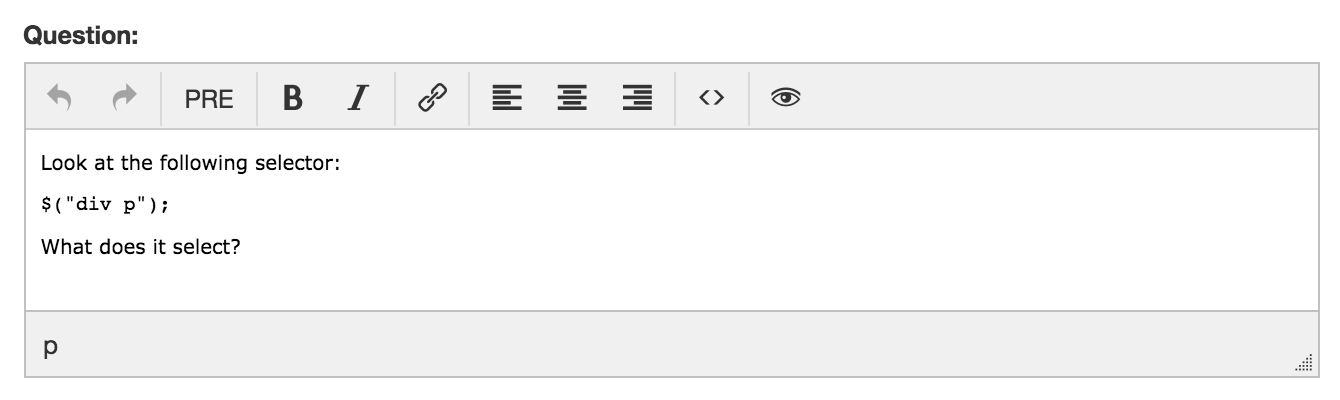
\includegraphics[width=\textwidth]{tinymce.png}
	\caption[TinyMCE]{TinyMCE editor as implemented in CRSFIT.}\label{fig:tinymce}
\end{figure}

\subsubsection*{Short URL}
To access a group directly it is necessary to know the URL. As a convenience, a url shortening feature is added to all groups using the \texttt{short\_url} library\footnote{\url{https://pypi.python.org/pypi/short_url}}. The url is not stored as persistent data, but simply generated on the fly. When a user makes a GET request to one of the shortened URL's the following method is hit.

\begin{lstlisting}[caption=The URL redirect method, label=lst:url-redirect]
@login_required
def url_redirect(request, short):
    group_id = short_url.decode_url(short)
    group = get_object_or_404(QuestionGroup, pk=group_id)
    return redirect(group)
\end{lstlisting}

The \texttt{short} parameter is the short key that is generated when a group is requested. Since we can decode it, it's possible to retrieve the group and redirect to it as shown in listing \ref{lst:url-redirect}. The url-shortening feature is provided as a convenience to allow students to easily access groups. The intention here was to make it as easy as possible to access a group of questions, to avoid possible confusion while navigating the interface.

\subsubsection*{Live updates}
Whenever someone answers a question the response can be seen live by the owner of the question at \texttt{.../question/<question-number>/responses/}. The graph will automatically update and display the current result. In order to show live updates we use Pusher. Pusher is a service for sending and receiving live data easily\footnote{Retrieved on 2016-04-04 \url{https://pusher.com/}}.
In order to use Pusher we create a channel to which we subscribe and bind an event to. This can be seen in \texttt{push.js} found in the vote app. The event that triggers Pusher is whenever someone answers a question. To tell Pusher, that there's a new event we trigger Pusher from the \texttt{answer\_response} view and provide it with the relevant data:

\begin{lstlisting}[caption=Selected parts of the answer\_response view, label=lst:answer_response]
        ...
        myData = {
            'total_responses': question_obj.total_responses(),
            'labels': [a.answer_text for a in answer_set],
            'series': [a.number_of_responses() for a in answer_set]
        }
        event = "response-%s%s%s" % (room, questiongroup, question)
        get_pusher().trigger('crs', event, {'data': myData})
    return redirect(qg)
\end{lstlisting}

The trigger at line 8 in listing \ref{lst:answer_response}, is where the view tells Pusher that there's a new event. From here, Pusher tells all subscribers of the corresponding channel, \texttt{crs}, that there's a new event which we can then handle. The event name should be unique, otherwise everybody will receive the same data. To ensure uniqueness we simply join each primary key for room, questiongroup and question into a string. This way we can separate responses from each other and ensure that graphs are not updated with data from other questions.
In \texttt{push.js} we do the following to subscribe and handle the events sent by the view:

\begin{lstlisting}[caption=Selected parts of push.js, label=lst:push.js]
var channel = pusher.subscribe('crs');
var event = $("#event:hidden").val();
channel.bind(event, function(data) {
    divs = $(".answer-box");
    divs.each(function(index, value){
        var answerId = parseInt($(value).attr('id'));
        var answer_count = data.data[answerId] ? data.data[answerId].answer_count : 0;
        $(value).text(answer_count);
    });
    $("#response-count").text(data.data.total_responses);
    chart.update(data.data);
});
\end{lstlisting}
The code in listing \ref{lst:push.js} subscribes to events on the channel named \texttt{crs} and handles updates to the response page by getting the data from the event and displaying it in the chart besides updating the number of total responses.


\subsubsection*{Deployment}
%\todo{Vi skal da have en oversigt over hvordan det er sat op på amazon med database server, S3 for static files osv. Tænkte jeg godt på :) Det kan vi jo sagtens, så kan vi bruge lidt fra Scalability faget OMG}

For deployment of the system we have chosen a 3-tier architecture. This consists of one web server, one media server and one database server as shown in figure \ref{fig:3-tier}. 

\begin{figure}[H]
\capstart
	\centering
		\includegraphics[width=7.5cm]{n-tier-diagram.png}
	\caption[]{The 3-tier architecture \label{fig:3-tier}}
\end{figure}

The web server is responsible for hosting Django and all the dynamic content, such as the HTML files. The media server is used to host static files, such as CSS, JavaScript and images. The database is hosted on a server of it's own, this allows us to easily add more web servers for scaling if needed.

The system is hosted using Amazon Web Services (AWS)\footnote{\url{https://aws.amazon.com/}}. The web server is an EC2 instance running Ubuntu 14.04 with Apache2 and Django installed. The Apache2 web server is installed with the \texttt{mod\_wsgi}\footnote{\url{https://modwsgi.readthedocs.io/en/develop/}} mod, to support Python WSGI applications.

The media server is an Amazon S3 bucket, containing all the static files. For the database, we are running an Amazon Relational Database Service (RDS) instance. Using RDS have several advantages. First, all data is separated from our web server. This makes horizontal scaling of the web servers very easy, since we simply need to add another copy of our EC2 instance to the cluster and add a load balancer in front of that, as shown in figure \ref{fig:n-tier}.

\begin{figure}[H]
\capstart
	\centering
		\includegraphics[width=9.5cm]{2-n-tier-diagram.png}
	\caption[]{The n-tier architecture \label{fig:n-tier}}
\end{figure}

Secondly vertical scaling is possible, since it is only a question of telling the EC2 instance to add more RAM, bigger CPU or whatever might be needed to gain more power \cite[p.~204]{henderson2006building}.

It would be ideal to run the n-tier setup from the beginning, since the 3-tier setup has one major fault, if one server fails, everything fails. There is no redundancy available, so we are vulnerable to potential full system failure. Even the n-tier setup shown in figure \ref{fig:n-tier} is not redundant enough, since there's still only one media server, and one database server. That means that even though we might be scalable in the terms of larger amounts of traffic, we are still vulnerable to system failures. If we needed to upgrade a server, only having one of each would possibly result in downtime. Having more would enable us to upgrade one node at a time, ensuring no downtime at all.

Currently memcached is running on the EC2 instance. This is not a viable solution if we were to scale the webservers horizontally. Depending on which server you get redirected to by the loadbalancer, potential cache inconsistency could occur. This is however easily fixed, by adding another server handling all the caching. We have added caching to prove a point, and are aware that this setup could be improved. The addition of a separate cache server however costs money by the hour, and has not been included.

% The most preferable mode of redundancy 
Since we are only using this for demo purposes, we have gone with the 3-tier setup as a minimum working solution, keeping the n-tier setup as a possible future architecture for a real production environment.






\subsection{Summary}
In the sections above we have described CRSFIT in detail. It's features, how it is developed, the tools used and the deployment process. To summarize all the features, compared to section  \ref{sec:competitor-overview}, we have added CRSFIT to the overview as shown in table \ref{tab:overview-2}.


\begin{landscape}
\thispagestyle{empty}
    \begin{center}
        \begin{table}[H]
            \begin{tabularx}{\paperwidth}{ |X|X|X|X|X|X|X|X|X| } 
             \hline
                 & Web \newline Software \newline Hardware based & Multiple question types & Multiline support & Mathematical notation & Source code notation & Supports image upload as questions & Timed questions/auto closing questions & Payment model \\ \hline
                 
              Kahoot                & Web   & No    & No    & \cellcolor{red!25}No    & \cellcolor{red!25}No    & Yes   & Yes   & Free \\ \hline
              Socrative             & Web   & Yes   & Yes   & \cellcolor{red!25}No    & \cellcolor{red!25}No    & Yes   & No    & Free \\ \hline
              Poll Everywhere       & Web   & Yes   & No    & \cellcolor{green!25}Yes   & \cellcolor{red!25}No    & No, only in answers   & Yes   & Subscription \\ \hline
              iClicker              & All   & Yes   & No    & \cellcolor{red!25}No    & \cellcolor{red!25}No    & Yes   & No    & Mixed based on solution \\ \hline
              Mentimeter            & Web   & Yes & No   & \cellcolor{red!25}No    & \cellcolor{red!25}No    & No    & Yes   & Subscription \\ \hline
              Tophat                & Web   & Yes & Questions only & \cellcolor{green!25}Yes & \cellcolor{red!25}No, only in questions   & No    & Yes & Subscription \\ \hline
              Learning Catalytics   & Web \newline Software   & Yes    & Yes  & N/A   & N/A   & Yes   & N/A   & Subscription \\ \hline
              Informa        & Software & Yes & Yes  & \cellcolor{red!25}No & \cellcolor{green!25}Yes, but only Java   & No    & No    & Research project, free \\ \hline
              Renaissance           & Software \newline Hardware & Yes & No & \cellcolor{red!25} No & \cellcolor{red!25}No & N/A & No & Hardware purchase \\ \hline
              Classroom Learning Partner & Software \newline Hardware & Yes & Yes & \cellcolor{red!25}No & \cellcolor{green!25}Yes & Yes & No & Research project, not available \\ \hline
              Shakespeak            & Software \newline Web & Yes & Yes & \cellcolor{red!25}No & \cellcolor{red!25}No & No & No & Subscription \\ \Xhline{2\arrayrulewidth}
              CRSFIT                & Web & No & Yes & \cellcolor{green!25}Yes & \cellcolor{green!25}Yes & No & No & N/A \\ \hline
            
            \end{tabularx}
            \caption{Updated overview of Classroom Response Systems}\label{tab:overview-2}
        \end{table}
    \end{center}
\end{landscape} \clearpage
% We have designed a test based on previous tests of response systems with the purpose of finding out if the systems is able to increase interaction in class. The test and the design of the test will be described in detail in this section.
\section{Testing classroom response systems in a classroom}\label{sec:testingcrs}
%The following sections will describe the methods we will use to test CRSFIT and the analysis of our results.
We have designed a test in order to determine if our solution can have a positive impact on teaching classes that covers teaching programming and mathematics. \citeA{siau2006use} found that there wasn't developed any instrument for measuring interactivity. This resulted in \citeA{siau2006use} to create their own method, from which we have taken elements to support our own.

%The following sections will also include the analysis of the results from our tests. 
With students from two different courses participating in our test, we will compare the results from each course, one using CRSFIT and one using Mentimeter. Qualitative results from our questionnaires will be examined in order to discover areas of the test and system which could be improved.




\subsection{Measuring interactivity}
The test by \citeA{siau2006use} is designed to tell whether or not they are able to move peoples behaviour, beliefs and attitude towards engagement, interactivity and participation during class. The test they designed consists of a \emph{pretest}, \emph{implementation} (of the system in a class) and a \emph{posttest} followed up by a \emph{qualitative data collection}. The pretest and posttest were made as questionnaires and the implementation was a hardware based CRS solution.

Our test is structured in the same way and we are asking similar questions in the different parts of the test as well. The whole test should preferably be carried out over a whole semester, but due to the limited time of this project the tests will be carried out in a single lecture in two different courses. The courses used in our tests was \emph{Frameworks and Architectures for the Web} (the Frameworks course) and \emph{Advanced Programming} (the Advanced course).

By having a pretest and a posttest asking the same questions \citeA{siau2006use} was able to compare the results and measure whether or not they were able to move peoples attitude. Their pretest consisted of two parts which were asking about individual interactivity and general interactivity in the class. The questions in both parts of the pretest were formulated as statements such as \emph{"I am engaged in class"} and \emph{"I provide my opinion to questions from the teacher during the class"}. This part of their test will be almost identical to our test. Our test primarily differs from theirs in the posttest. Since we are not able to carry out our test over a longer period of time, our posttest will not be asking into \emph{individual interactivity} and \emph{general interactivity} again. We will, however, use the results from \emph{individual interactivity} and \emph{general interactivity} from the pretest to tell to which degree students interact in class in general. The pretest should be answered by students before or in the beginning of the given lecture in which the test is carried out (See appendix \ref{app:pretest} for the complete list of questions from the pretest questionnaire).

During the lecture of the Frameworks course we asked students questions relevant to their class using our solution, CRSFIT. This part of the test is the \emph{implementation}. Students answered the questions anonymously and they were not held accountable. The purpose of this part of the test is to 1) tell if students actually benefit from using the system and overall find it useful, and 2) test our solution in a real setting.

It requires training and experience to get the most out of a classroom response system. The literature and insights about how to use response systems in a beneficial way has developed alongside with the research of the implementation of response system in classrooms. For example, see: \cite{lantz2014effectiveness,draper2004increasing,lin2011implementing} for insights and comments about how to effectively use response systems. 
We have developed questions for the Frameworks course in collaboration with our supervisor, Peter Eklund, which was asked during the lecture in which we carried out the test.
The questions that where asked during the test in the Frameworks course can be found in appendix \ref{app:questions} and on the live site at \url{http://crsfit.online/r/b4tc8} (login required). 

The questions asked in the Advanced Programming course, was developed by the course teacher, Andrzej Wasowski and can be found in appendix \ref{app:questions-advanced}.


\subsection{Acceptance of technology}
In the posttest questionnaire we ask students about the perceived ease of use of CRSFIT and the perceived usefulness. The \emph{perceived ease of use} is included in the test in order to get feedback on how easy the system is to use. The \emph{perceived usefulness} asks into the idea and possible benefits of the system with statements like \emph{"Using the system makes it easier for me to interact in the class"} to be rated. Perceived ease of use and perceived usefulness is adopted from the \emph{Technology Acceptance Model (TAM)} \cite{siau2006use,davis1989user} where they are defined as follows:

\emph{"Perceived usefulness (U) is defined as the prospective user's subjective probability that using a specific application system will increase his or her job performance within an organizational context. Perceived ease of use (EOU) refers to the degree to which the prospective user expects the target system to be free of effort."} \cite[p.~985]{davis1989user}.

The model originally aims to predict users intention to adopt new technology. Inspired by the questions in a different research project by \citeA{davis1989perceived} we will ask similar styled questions in our posttest.

This part of the test will tell if the students feel an individual increased interactivity by using our system. Also, we ask the students whether or not they use any tools to test their answers which includes code/script or mathematical expressions. Included in the posttest questionnaire is also an open ended question in which we ask students to give their opinion about advantages and disadvantages of using a classroom response system. This is the qualitative part of the test. This part serves to give us an idea about areas that this kind of system does particular good or bad. See appendix \ref{app:posttest} for a complete list of the questions from the posttest questionnaire.


\subsection{The pretest and posttest questionnaires} % Field testing the system with quantitative and some qualitative data
% Likert scale
% Spørgsmål - se bog. Structured format (i form af at spørgsmålene ikke bliver spurgt af os, men står på tekst (spørgeskema). Likert skala, 1-9. (Find artikel)
% Open ended spørgsmål til at slutte af med - kvalitativ data som vi vil bruge til ?? i analysen.
The pretest and the posttest are designed as questionnaires. Questionnaires makes the least demands on personal and social skills of the questioner \cite[p.~74]{deacon2007researching} and enables us to measure the results. The questionnaires are to be answered online using Google Forms\footnote{\url{https://www.google.dk/intl/da/forms/about/}}. Our way of asking the questions are highly structured since they are written down (using Google Forms) and asked in the exact same way to all participants \cite[p.~65]{deacon2007researching}. Both questionnaires can be found in the appendix (\ref{app:pretest}, \ref{app:posttest}).

When asking questions in a questionnaire (or in general) the questioner should be aware which type of questions are asked. What does the question seek to find information about? \citeA[pp.~80-84]{dillman1978mail} lists four types of questions which are asking into either \emph{behaviour}, \emph{beliefs}, \emph{attitudes} or \emph{attributes}. With our questions we are interested in behaviour, beliefs and attitudes. We are not focusing on attributes. Questions asking into attributes are concerned about background information of the respondent such as age, gender etc. \cite[p.~75]{deacon2007researching}. While these questions typically are easy to answer, they are of no interest to us. They are often used to say something about a group of people you don't know and are of most use in very large samples. Our questions are interested in behaviour when we ask student to rate statements such as \emph{"I interact with the teacher in class"} and beliefs (\emph{"Students receive feedback from the teacher during the class"}) and attitudes (\emph{"I find the system useful in enhancing my interaction in the class"}).

It may seem that some of our questions are identical to each other even though they are slightly different. Because of this we risk that respondents doesn't see the difference from the previous question and therefore may answer the same as in the previous question. Because of the similarity we could risk that respondents find the questionnaire as a whole to be frustrating or difficult to answer.

All of the questions in our questionnaires (except two) are formulated as statements which should be answered on a Likert scale \cite{likert1932technique} with items 1-9 where 1 is \emph{Strongly disagree} and 9 is \emph{Strongly agree}. With an uneven number we offer a neutral choice (5 on our scale) in order to avoid forcing an opinion on the respondents. We could have chosen to make the scale smaller or larger. A smaller scale than 1-9 could result in less different answers since the options are fewer. \citeA[p.~507]{matell1972there} found that less than 7 options on a Likert scale resulted in greater usage of the "neutral" choice. %In order to avoid that we choose 9 options which we hope will not offer too many options as well.


%To sum things up the following list shows what we'll do and when:

%\begin{itemize}
%    \item Pretest: Questionnaire, before or in the beginning of the lecture
%    \item Implementation: Students answer questions with CRSFIT during lecture
%    \item Posttest + qualitative data: Questionnaire, in the end of the lecture
%\end{itemize}

\section{Results}

The two tests were carried out in a classroom setting in two different courses, \emph{Advanced Programming} and \emph{Frameworks and Architectures for the Web}. All students in each class were given the pretest and the posttest, and used a CRS system in between. The Advanced course used Mentimeter, and have done so throughout the semester. The Frameworks course used our system, CRSFIT, and have not used any other CRS throughout the course.
There were 10 students out of a total of 42 enrolled present while performing the tests in the Frameworks course. This resulted in 8 responses in the pretest (N1 = 8), and 10 in the posttest (N2 = 10). The pretest was send out to students before class, and they were given 5 minutes to answer it first if they had not done so already.
In the other course, Advanced Programming, there were 50 students present while performing the tests out of a total of 89 students enrolled in the course. This resulted in 48 responses in the pretest (N3 = 48) and 50 in the posttest (N4 = 50). 
The raw data from the questionnaires can be found in appendix \ref{app:data}.

\subsubsection*{Individual and general interactivity}\label{sec:individual_and_general}

% Pretest
Within the pretest we asked students about \emph{Individual interactivity} and \emph{General interactivity}. When students are asked to assess their own interactivity they tend to rate it lower than when they are asked to assess the general interactivity. The average for individual interactivity was $5,99$ compared to $6,11$ for general interactivity in the Frameworks course. For the Advanced course it was $5,23$ compared to $6,25$. 

%They also asked into individual and general interactivity again after implementing a CRS into a class and found that the students assessed the individual and general level higher (6.8 and 7.1 respectively). Side 400. Statistisk signifikant. Til diskussion. 

The individual interactivity shows if students believe they are active during a lecture. Both the Advanced and Frameworks course had two hours of lecture, and two hours of lab support, for a total of 4 hours of class. Figure \ref{fig:individual_interactivity} shows the similarities and differences in student's individual interactivity in class in both courses.

 \begin{figure}[H]
  \centering
     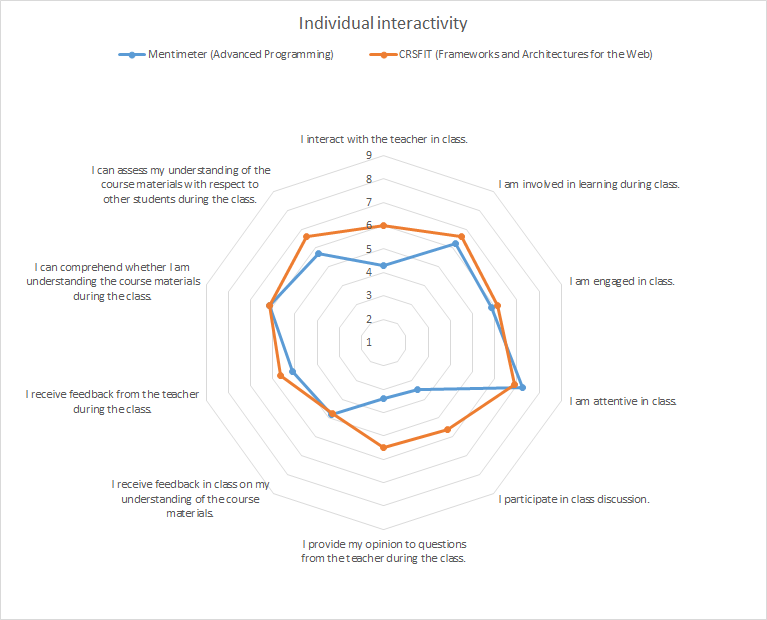
\includegraphics[width=\textwidth]{./individual_interactivity.png}
     \caption{Pretest - Individual interactivity}
     \label{fig:individual_interactivity}
 \end{figure}

The biggest difference is found in the questions \emph{I participate in class discussion} and \emph{I provide my opinion to questions from the teacher during the class}. These questions are very specific to taking part in class and actively participating, where other questions like \emph{I am involved in learning during class}, might not necessarily imply any direct focus on the individual student. 

%Reasons for these variations could be found in the course differences. Advanced Programming has formal prerequisites where you must be able to program, know basic functional programming, discrete mathematics and more. The Frameworks course is an introductory course so it has no formal prerequisites. Based on this, the learning curve could be steeper in the Advanced Programming course since it is considered an advanced curriculum, and therefore less people might participate in class discussions since the subjects discussed might be harder to comprehend at first. Also course size might have influenced the outcome. The Advanced course has more than twice as many students enrolled as the Frameworks course (89 vs. 42), here students might hold back their participation due to the large amount of people or there simply may not be enough time to have all students participate.

The responses to the question \emph{I interact with the teacher in class} also has a large difference with a mean of $6$ in the Frameworks course versus $4,29$ in the Advanced course. 

%Again this outcome can most likely be explained by a larger class and tougher topics that take longer to discuss and understand. It might also involve the teachers style, where some might include students more, and some less. A point to notice though, is the fact, that the scores are on each side of the neutral value 5. Where $4,29$ is slightly more towards disagreeing and $6$ is the other way around.

The general interactivity shows how students think others interact in the course. Compared to the individual interactivity the results from general interactivity are much more aligned as mentioned above. The highest differences are found in the statements \emph{Students interact with the teacher in class} and \emph{Students are involved in learning during class}. Comparing the mean of the two courses shows a difference less than 1. Overall the attitude towards general interactivity is very close to each other in both courses. Results for both courses are shown in figure \ref{fig:general_interactivity}.

 \begin{figure}[H]
  \centering
     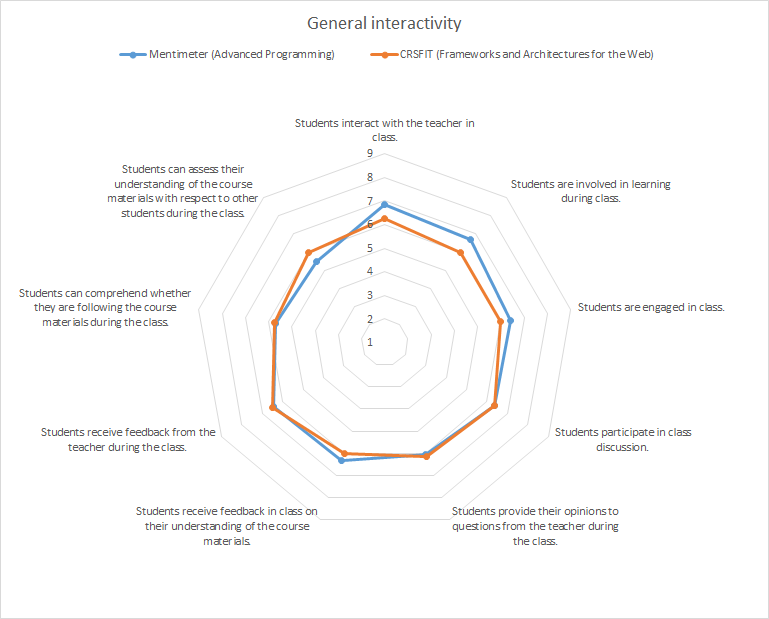
\includegraphics[width=\textwidth]{./general_interactivity.png}
     \caption{Pretest - General interactivity}
     \label{fig:general_interactivity}
 \end{figure}

Comparing individual and general interactivity in both courses on the similar statements \emph{I participate in class discussion} and \emph{I provide my opinion to questions from the teacher during the class} (figure \ref{fig:individual_interactivity}) to \emph{Students participate in class discussion} and \emph{Students provide their opinions to questions from the teacher during the class} (figure \ref{fig:general_interactivity}), shows that when students are asked to assess themselves, they rate lower, than when asked to assess others. The statements mentioned are the ones with the biggest differences in their answers when asked about individual interactivity but they are exactly the same when asked about general interactivity. This suggest that a small group of people participate in the discussions often, so the general picture is good, but the individual might not be. 


% last two questions of the pretest
A relatively large amount of the students answered 5 to the last two questions in the pretest. The questions states: \emph{Students can comprehend whether they are following the course materials during the class} and \emph{Students can assess their understanding of the course materials with respect to other students during the class} (appendix \ref{app:pretest-general}, item 8 and 9). 
In the first question 15 out of 48 students from the Advanced course answered 5. In the second question 16 students answered 5.
In the Frameworks course, 4 out of 8 students answered 5 in the first question, and 4 students answered 5 in the second question.



%The large amount of neutral responses could suggest that these could be statements which are difficult to assess. Another explanation could be that these statements are the very last in the pretest and students could be bored at this point and just answer 5 to whatever they are asked to assess. Or it could be that a large amount of the students have a neutral opinion to the statements. Either way, the results stands out from the rest with a relatively large amount of neutral answers.


\subsubsection*{Ease of use and perceived usefulness}
% Posttest, mean of Ease of use	and Perceived usefulness
In the posttest we asked the students to assess the \emph{ease of use} and \emph{perceived usefulness} of the CRS they were using. The overall mean of \emph{ease of use} for CRSFIT is $7,8$ and for \emph{perceived usefulness} it is $6,7$, compared to Mentimeters $8,1$ and $8,3$ respectively. A mean for each statement is shown in figure \ref{fig:perceived_ease_of_use_and_usefulness}.

 \begin{figure}[H]
  \centering
     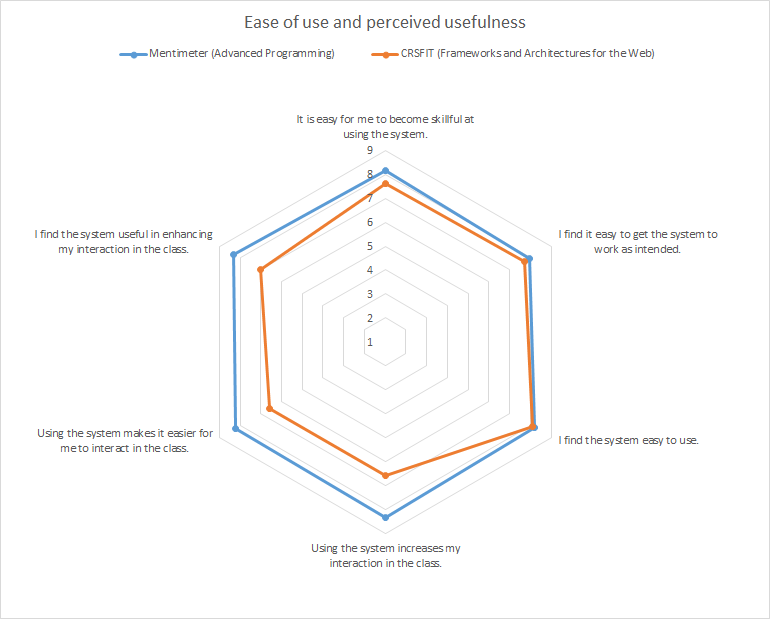
\includegraphics[width=\textwidth]{./perceived_ease_of_use_and_usefulness.png}
     \caption{Posttest - Ease of use and perceived usefulness}
     \label{fig:perceived_ease_of_use_and_usefulness}
 \end{figure}
 
The relatively high value of \emph{ease of use} suggests that the students found CRSFIT easy to use to an extend that is closely comparable to Mentimeter. The overall \emph{perceived usefulness} for CRSFIT was found to be $6,7$ which is in the upper third quartile of the scale. For Advanced Programming the overall \emph{perceived usefulness} was found to be $8,3$. 


%The lower level of perceived usefulness compared to Mentimeter could be explained by the way the test was carried out. The results may have been different if the test was carried out over a longer period of time during regular lectures. For example, students might be more convinced that a CRS is useful if they have used it over the course of a whole semester, and therefore rate the perceived usefulness higher. This is compared to testing CRSFIT in just one lecture, where the system is new to them. As mentioned, the class using Mentimeter have had the chance to get well acquainted with the system before doing our test.

As an addition to the test we asked the students whether or not they ran and tested their solutions for the questions they were asked (appendix \ref{app:posttest-open-ended}, item 2). Both the Advanced and Frameworks course were asked questions that included code. We found that only 16\% of students from the Advanced course answered that they ran the code from the questions while 60\% of the students from the Frameworks course answered that they ran the code from the questions. 

%The result from the Advanced course is surprisingly low considering they have used Mentimeter from the beginning of the semester. However, they may have responded relatively to the lecture in which the test was carried out. At the time the test was carried out, the class has been using a REPL (Read–Eval–Print Loop) for Scala, an interactive command line tool for easily running code, for several months.


%During the test in the Frameworks course, one person mentioned that question 6 (appendix \ref{app:questions}, item 6) was a math question. The question could be asked in any programming language and is not jQuery specific as many of the other questions. This particular question was designed to force the students to run the code since it otherwise would be hard to figure out the correct answer. At this point in the test, it was proposed that in order to answer the question, the students could simply run the code and get the answer. This could be an explanation why 60\% of the students from the Frameworks course answer that they ran the code from the questions. If it had not been brought up during the test, then fewer students might have answered that they ran the code. Despite being brought up how to answer question 6, one still failed to provide the correct answer.

%Another important note on the difference between the two courses on whether or not they ran the code from the questions could be the availability of the code. Mentimeter was used by presenting the questions and answers in a separate slideshow and thus not entered into Mentimeter (because of the systems limitations). If these slideshows weren't available to the students during lectures, then copy-pasting the code into a REPL would not be an option and manually writing the code may be too much an effort in order to test the code from the questions. CRSFIT, on the other hand, provides the code and is easily copy-pasted.


\subsubsection*{Qualitative part of the test}
In the posttest we asked both students from the Advanced and Frameworks course about the advantages and disadvantages of using a classroom response system. Since the students from Advanced Programming used Mentimeter their comments must be seen in relation to this, also they have been using it from the very beginning of the semester, so they have more experience with classroom response systems in general. The overall picture from the comments is that the students from Advanced Programming seems pleased with using the system.

One student points out a disadvantage when saying \emph{"[a] Disadvange could be that people might not get the help they need during Classes."} (appendix \ref{app:qualitative-advanced}, item 25). 
%If the time using a CRS is taken from helping students individually, then it could be a disadvantage. However, it will often be the individual teacher's responsibility to manage the time in the courses they teach. Another student mentions awkward pauses when using Mentimeter (appendix \ref{app:qualitative-advanced}, item 13). This may however be the same for every CRS and depends on how the teacher uses the system.
Among many of the advantages reported by the respondents from Advanced Programming is increased attention, more interaction (appendix \ref{app:qualitative-advanced}, item 4, 6, 10, 12, 13, 14) and forced thinking with feedback (appendix \ref{app:qualitative-advanced}, item 11, 16, 17, 19, 20, 22). These advantages are just some of the advantages any CRS should provide when used properly. The overall impression from Advanced Programming is that they found Mentimeter useful, which is also the impression we get when looking at the perceived usefulness in figure \ref{fig:perceived_ease_of_use_and_usefulness}, where they report an average score greater than 8. This is a better score than the one reported by the students from the Frameworks course, which was $6,7$. Their comments somewhat reflect that as well, where they tend to be about the situation in which the test was carried out (appendix \ref{app:qualitative-frameworks}, item 1-4). Also, there was no mentioning of code being presented in slideshows rather than in the actual CRS (Mentimeter) found in any of the comments from the students in the Advanced course.

%As highlighted by some of the respondents in the posttest from the Frameworks course, there's room for improvement when using CRSFIT. The way the test was carried out didn't resemble a regular lecture enough. As mentioned earlier in chapter \ref{sec:testingcrs}, teaching and using a CRS requires training and experience. The test of the system was not carried out in a regular lecture by a teacher as it would have been if it was a normal setting. The test was carried out by us, letting people answer one question at a time. Normally, a teacher might ask one or two questions after a period of time with lecturing in between or after finishing a subject, and not ten questions in a row as it was the case in our test.

Two respondents from the Frameworks course answered that they would like to wait before seeing what other students answered. As one points out: \emph{"Students are easily biased, and it is hard to not look at what everyone else has answered before answering yourself."} (appendix \ref{app:qualitative-frameworks}, item 4). For most questions in the test, the majority answered correctly except for in the very last question. This particular question was made harder and more comprehensive on purpose. See appendix \ref{app:questions} item 10. 
%The question got 8 responses and only two of them were correct. This may be because one of the first answers was incorrect and most people just followed along due to the difficulty of the question. The respondents that stated, they wanted to wait some time before revealing answers may have a point. If we waited some time before showing the responses for each question, we might have seen a larger spread in answers or maybe more correct answers in questions like the last one, because students would individually take the time to come up with an answer. 

One respondent points out that CRSFIT de-personalizes the connection between teacher and student and another says it results in less individual feedback (appendix \ref{app:qualitative-frameworks}, item 3 and 4). 
%This was the case in our setting. A teacher may go more into detail why one answer is correct and another isn't. Maybe a teacher would ask the students why an answer is (in)correct and use the system to start a discussion. This way the personal connection could be maintained for people who are used to interact in class while people not used to interact in class would be included as well through the system. In our case we briefly discussed some of the questions during the test, and did not go into depth about why an answer was correct or incorrect.

%One comment states that \emph{"it really helps examining yourself and seeing what you got or didn't get- at real time."} (\ref{app:qualitative-frameworks}, item 1). If students using our system immediately sees this advantage then we've come far. All of our questions were centered around topics covered in the course \emph{Frameworks and Architectures for the Web} in which our test was carried out. All of the questions and answers included code in a few different ways and we aimed at asking questions which they should be able to answer if they had followed the course. The comment implies we did that. 

%\todo{Smooth transition}
\subsubsection*{Summary of results}
The results reveals only a few noticeable differences in the comparison, which we will discuss further in the following section. It also revealed many results which are close to identical in the two courses. Among the comments from the students are various points which we will take into consideration in the discussion. The validity and how we can use these results will also be discussed in the following section.
 \clearpage
\section{Discussion} \clearpage
\section{Conclusion} \clearpage


%--------------------REFERENCES--------------------%
\bibliographystyle{apacite}
\bibliography{references.bib}
%--------------------REFERENCES--------------------%

\end{document}
